\chapter{Machine Learning Techniques}

\section{Dimensionality reduction}
Dimensionality reduction is the process of reducing the amount of features used in machine learning algorithms. This can be used to increase the accuracy and the performace of machine learning algorithms. One form is to do data compression. For example, transform 3D data into 2D data and eliminate a feature or dimension. It can also be used to reduce dimensions to be able to efficiently visualise data.\\\\
Dimensionality reduction can be used to speed up the time it takes for other learning algorithms to learn. By using dimensionality reduction, the amount of features or the amount of training samples is reduced which reduces the running time of the training, but the compressed data still retains the same information as the uncompressed data.

\subsection{Principle Component Analysis}
Principle Component Analysis is a way to do dimensionality reduction. The algorithm is formulated as a minimalisation problem. When given N-dimensional data and N-1 dimensional data is prefered, the algorithm tries to find the correct N-1 dimensional value so that the projection is the closest to the original data. \\\\
Before this algorithm is run, the features of the data should be scaled, so that all features are on a similar scale. This can be done by using mean normalization. In order to reduce the dimension from $n$ to $k$ the covariance matrix should be computed. \\\\
From this matrix, the eigenvectors need to be computed using singular value decomposition. From these values, only the first $k$ values are going to be used and be multiplied with the training data.

\section{Anomaly detection}
Anomaly detection is also a form of unsupervised learning. The algorithm learns what normal behaviour looks like through the training set and then tries to predict if a given input data belongs to the normal behaviour or is abnormal for any reason. \\\\
In Figure~\ref{fig:anomalydetection}, the algorithm has been trained using the green data points. These make up the normal behaviour. The algorithm can then predict whether a data point is normal, or an anomaly. It seems very close to One-class SVM's as seen in Section~\ref{oneclassSVM}. However, One-class SVM's are used for simple binary classification. Normal behaviour of a systems typically does not fall within a single class. Usually many different classes make up normal behaviour. 
\begin{figure}[H]
\centering
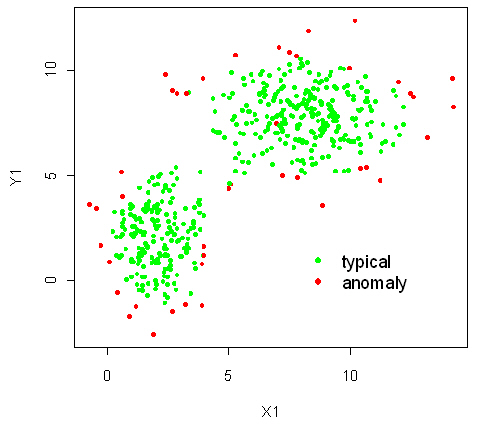
\includegraphics[width=0.8\textwidth]{Figures/anomaly}
\decoRule
\caption[Anomaly detection]{Anomaly detection. \cite{anomaly-fig}}
\label{fig:anomalydetection}
\end{figure}

\noindent Anomaly detection is useful when there are a lot of data points belonging to normal behaviour and there are almost no abnormal behaviour data points. General supervised learning algorithms are usefull when there are a lot of data points of both normal and abnormal behaviour. \cite{anomalyCoursera}

\subsection{Normal Distribution}
\noindent Anomaly detection algorithms make heavy use of (Gaussian) Normal distribution:
\begin{align}
x \sim N(\mu, \sigma^2)
\end{align}
Hereby $\mu$ is the mean parameter and $\sigma$ is the standard deviation. Now the probability of $x$ being an anomaly can be calculated as:
\begin{align}
p(x) = \prod_{j=1}^n( p(x_j ; \mu_j, \sigma_j)  ) \\
p(x_j ; \mu_j, \sigma_j) = \dfrac{1}{\sqrt{2\pi}\sigma_j} exp(- \dfrac{(x_j - \mu_j)^2}{2\sigma_j^2}) 
\end{align}
\noindent $p(x_j ; \mu_j, \sigma_j)$ is the probability of $x_j$ with a Normal Distribution with parameters $(\mu_j, \sigma_j)$. $p(x)$ is the product of all these probabilities. The formula for the probability is the probability density of the Normal distribution. This function is plotted in Figure~\ref{fig:normalExample}. The $y$-axis is the density function, the $x$-axis is the $x$ value in the formula. 

\begin{figure}[H]
\centering
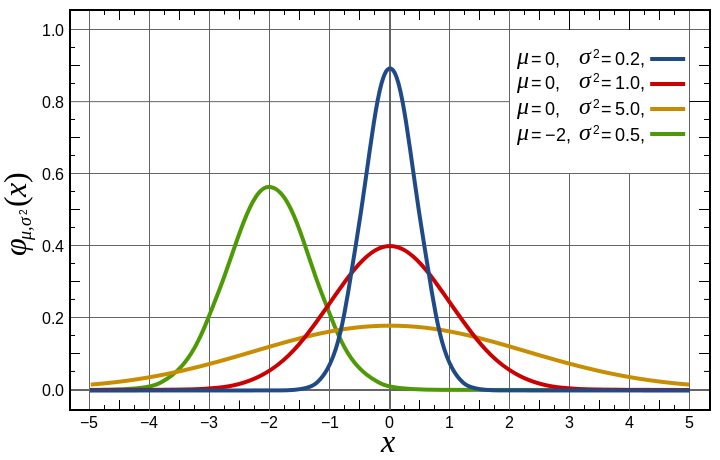
\includegraphics[width=0.8\textwidth]{Figures/normaldist}
\decoRule
\caption[Normal Distribution]{Normal Distribution. \cite{normalExample}}
\label{fig:normalExample}
\end{figure}

\section{Online learning}
Online learning is a technique to update an algorithm. Instead of feeding all data to the learning algorithm, the data is fed incrementally. The algorithm can keep learning from data even after it has initially learned a model. \\\\
Some algorithms such a KNN are immediatly able to do online learning. Other algorithms, such as SVM need to be slightly altered in order to be able to do online learning. \\\\
Online learning is very useful when the data is dependent on the time. For example, stock prices prediction. The data that is used to train an algorithm today might be able to predict stocks for tomorrow, but it is not very effective at prediction the stock market at long term. That is why it is useull to be able to keep training the algorithm. \cite{onlineLearning}

\section{Bagging}
Bagging is a technique which tries to create new datasets from a given data set. It takes a data set as input and generates multiple slight variations of the original data set. One method to do this is by generating a new dataset by sampling with replacement. \\
\\
This means that to construct a new dataset of size $n$, $n$ elements are chosen from the original dataset and that doubles are allowed. These slight variations will have a different distribution of samples in the dataset. This has as effect that the learning algorithm is trained differently. This method is also called Bootstrapped Aggregation, or bagging for short. \\
\\
Once multiple data sets have been generated, it is possible to combine multiple weaker models and training algorithms and try to combine the predictions made by these algorithms. This is useful to deal with unstable data. Unstable data is data that can give different results depending on the algorithm that is used to process the data. An example of bagging and Neural Networks can be seen in Figure~\ref{fig:baggingExample}. \cite{mlcat}

\begin{figure}[H]
\centering
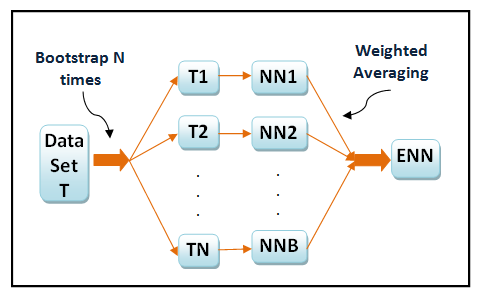
\includegraphics[width=0.8\textwidth]{Figures/bagging}
\decoRule
\caption[Bagging example with Neural Networks]{Bagging example with Neural Networks. \cite{baggingExample}}
\label{fig:baggingExample}
\end{figure}